\chapter{IMPLEMENTATION}

\section{Introduction}
The implementation phase involves translating the system design into a working web application. CivicGuard is built using the **Laravel 11.x** framework, which follows the Model-View-Controller (MVC) architectural pattern. This separation of concerns allows for modularity, scalability, and ease of maintenance. The backend is powered by PHP 8.2 and PostgreSQL, while the frontend is crafted with Blade templates and Tailwind CSS.

\section{Core Technologies Stack}
\begin{itemize}
    \item \textbf{Backend:} PHP 8.2 with Laravel Framework.
    \item \textbf{Frontend:} HTML5, Tailwind CSS, Blade Templates.
    \item \textbf{Database:} PostgreSQL 14.0 for persistent storage.
    \item \textbf{Package Management:} Composer (PHP) and NPM (JavaScript).
    \item \textbf{Environment:} Laravel Herd / PHP + PostgreSQL (Local Development) / Ubuntu Nginx (Staging).
\end{itemize}

\section{MVC Pattern Implementation}

\subsection{Database Models (`app/Models`)}
Models represent the data structure and business rules. The `Report` model handles relationships with the `User` model and defines the core logic for status transitions and photo handling.
\begin{lstlisting}[style=phpstyle]
// app/Models/Report.php logic snippet
public static function getCategoryDepartmentMap()
{
    return [
        'Road Damage' => 'Engineering & Public Works Department',
        'Clog Drains' => 'Public Health Department',
        'Street Light Not Working' => 'Electrical Department',
        'Waste Disposal' => 'Sanitation Department'
    ];
}
\end{lstlisting}

\subsection{Business Logic via Controllers (`app/Http/Controllers`)}
Controllers bridge the gap between models and views, following the "Thin Controller, Fat Model" philosophy. The `ReportController` manages the critical `store` method, which performs multi-file validation (ensuring only images are uploaded), generates unique file paths for local storage, and triggers the `ReportRoutingService`. For officers, the controller handles the ingestion of resolution photos and the final status update, ensuring that all actions are attributed to a specific authenticated user session.

\subsection{Unified View Components (`resources/views/components`)}
To maintain a premium, consistent look throughout the application, we implemented a custom component system using Blade. Navigation bars, input fields, and dashboard cards are abstracted into singular files. This allows us to update the primary CivicGuard accent color globally by changing a single CSS class, ensuring the UI remains agile and maintainable as new features are added.

\section{Security Implementation}
\begin{itemize}
    \item \textbf{Bcrypt Hashing:} All user passwords are salt-hashed using Bcrypt, ensuring that user credentials remain secure even in the event of a raw database compromise.
    \item \textbf{RBAC Middleware Stack:} Custom middleware (e.g., `verifiedOfficer`) acts as a security perimeter. It intercepts every request to the administrative routes, validating that the user has the correct permissions before any data is processed.
    \item \textbf{CSRF & XSS Mitigation:} Built-in protection against cross-site request forgery and cross-site scripting is enforced on every form. Laravel's Blade handles automatic escaping of data, preventing common frontend vulnerabilities.
\end{itemize}

\section{UI Implementation Screens}

\subsection{User Authentication Interfaces}
The login and registration screens are designed to be clean and inviting, following modern UI best practices.

\begin{figure}[H]
    \centering
    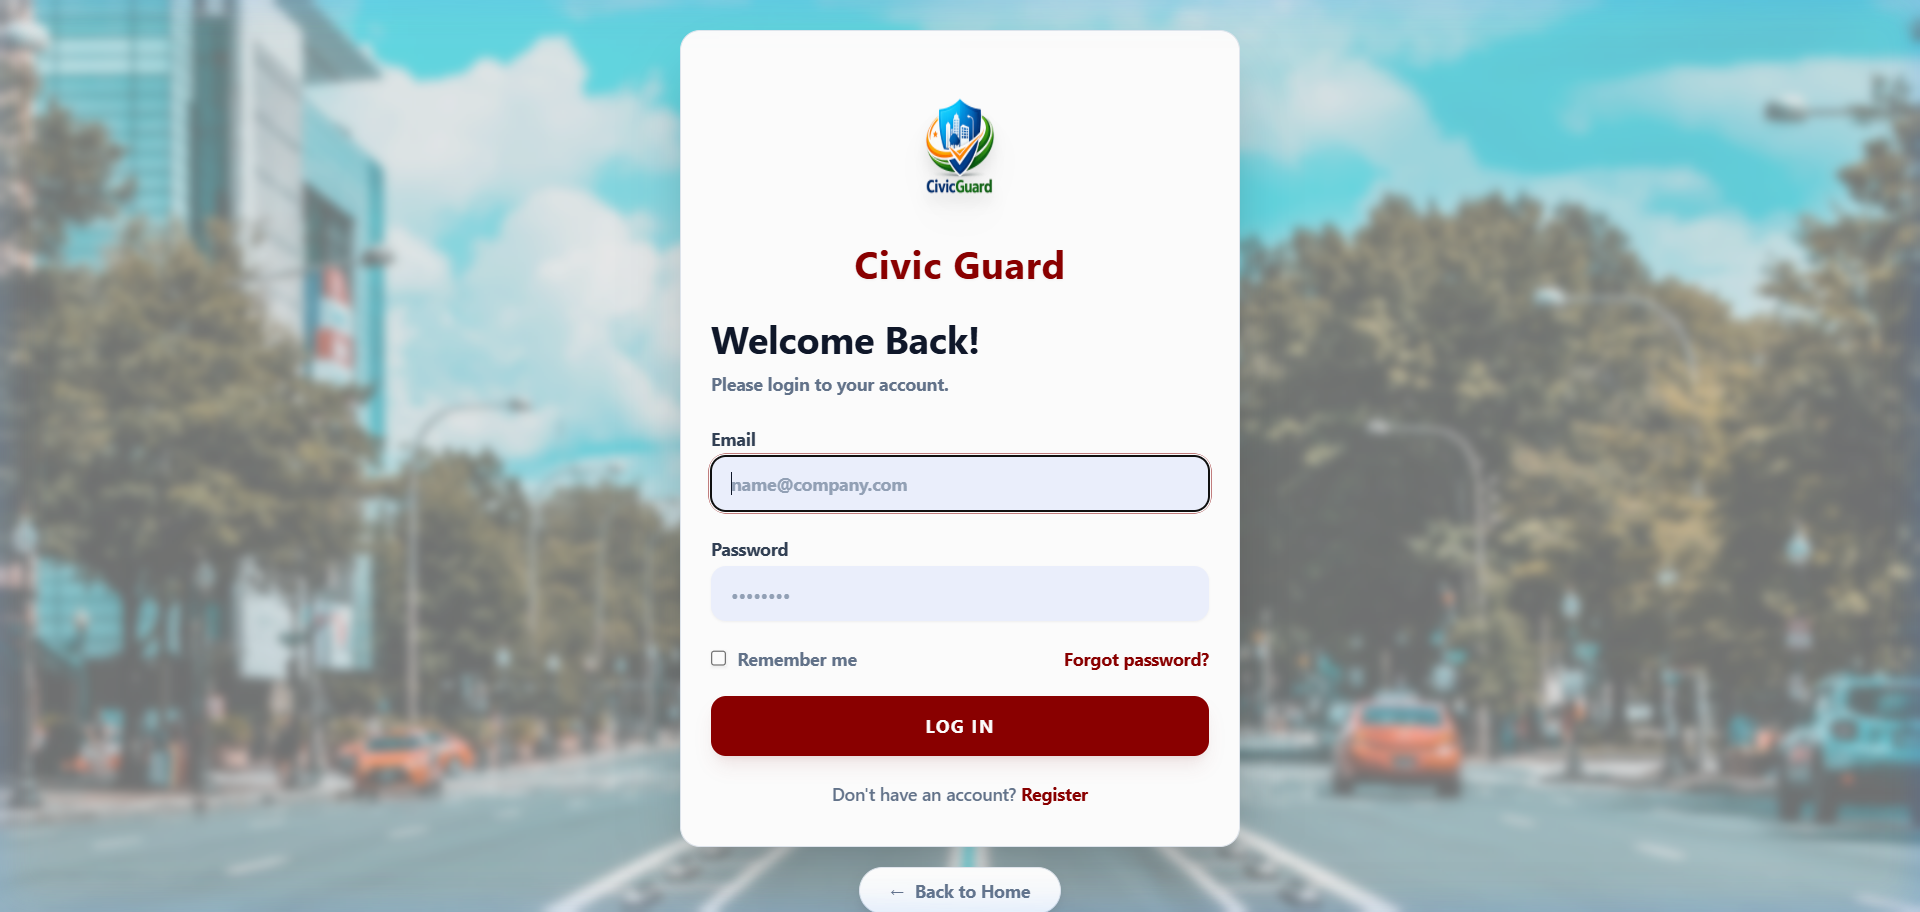
\includegraphics[width=0.9\textwidth]{images/login_page.png}
    \caption{Implementation - Secure Login Interface}
\end{figure}

\begin{figure}[H]
    \centering
    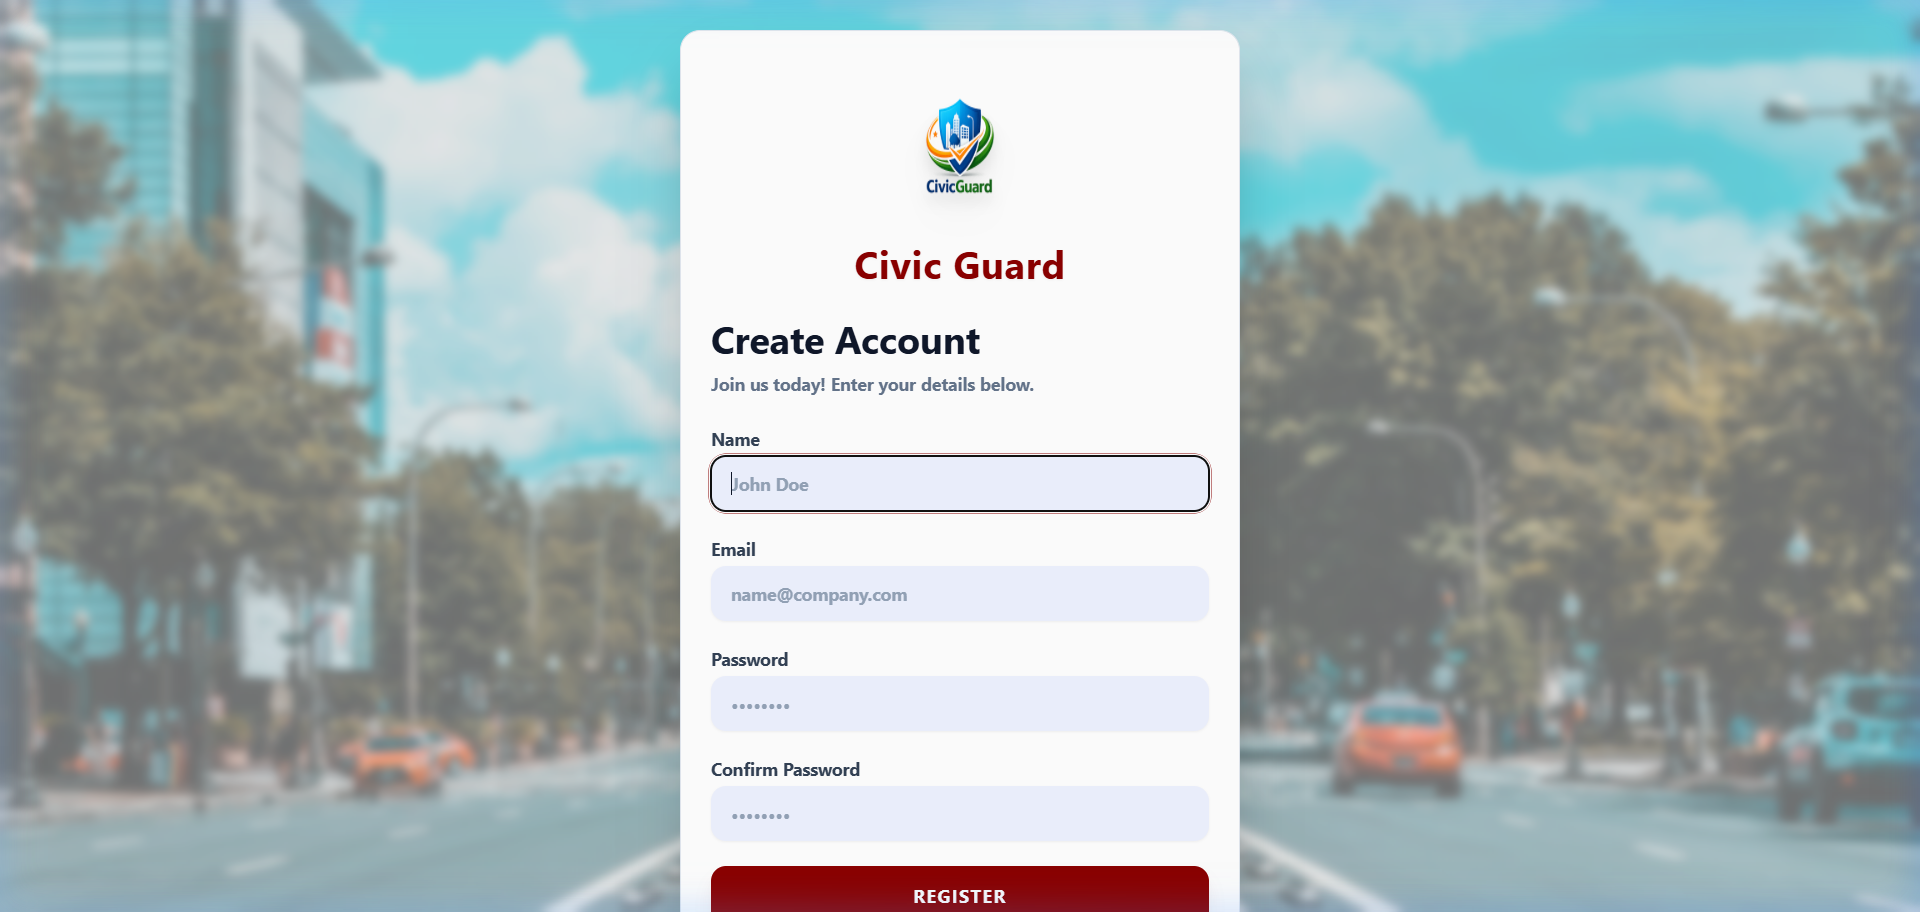
\includegraphics[width=0.9\textwidth]{images/register_page.png}
    \caption{Implementation - Citizen Registration Interface}
\end{figure}

\subsection{Project Dashboards}
The dashboards are the central hubs for all user interactions, providing immediate access to critical data.

\begin{figure}[H]
    \centering
    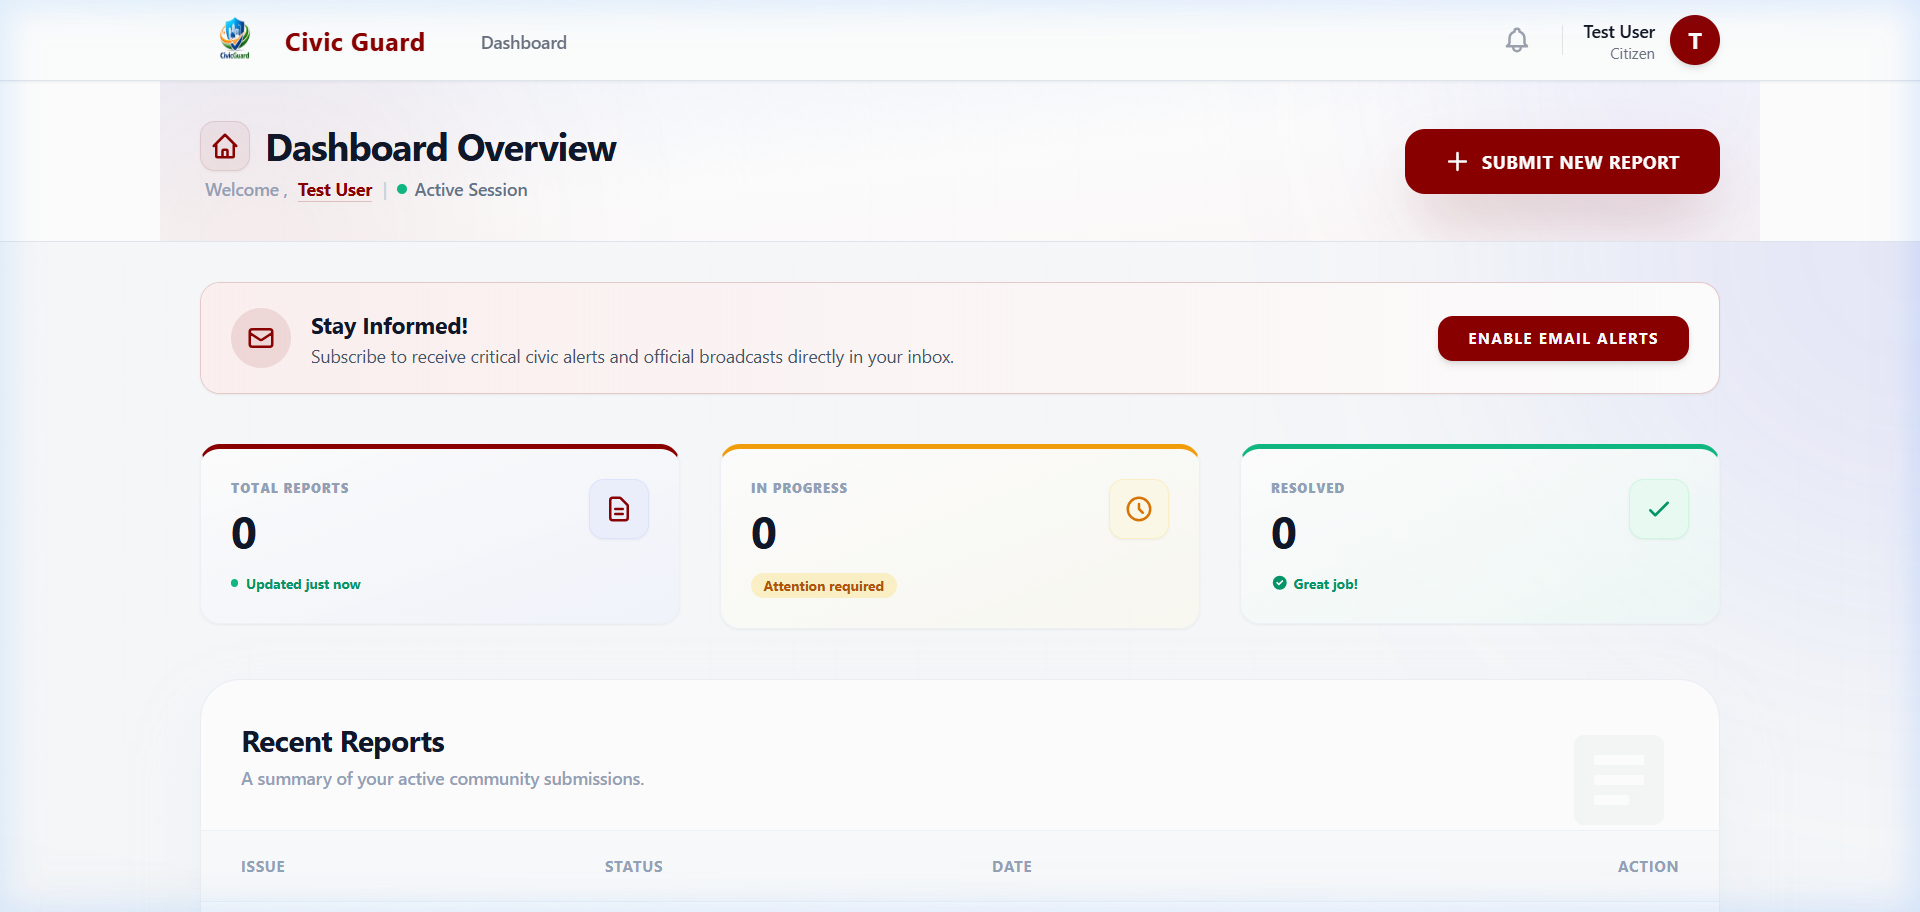
\includegraphics[width=0.9\textwidth]{images/dashboard.png}
    \caption{Implementation - Citizen Dashboard Overview}
\end{figure}

\begin{figure}[H]
    \centering
    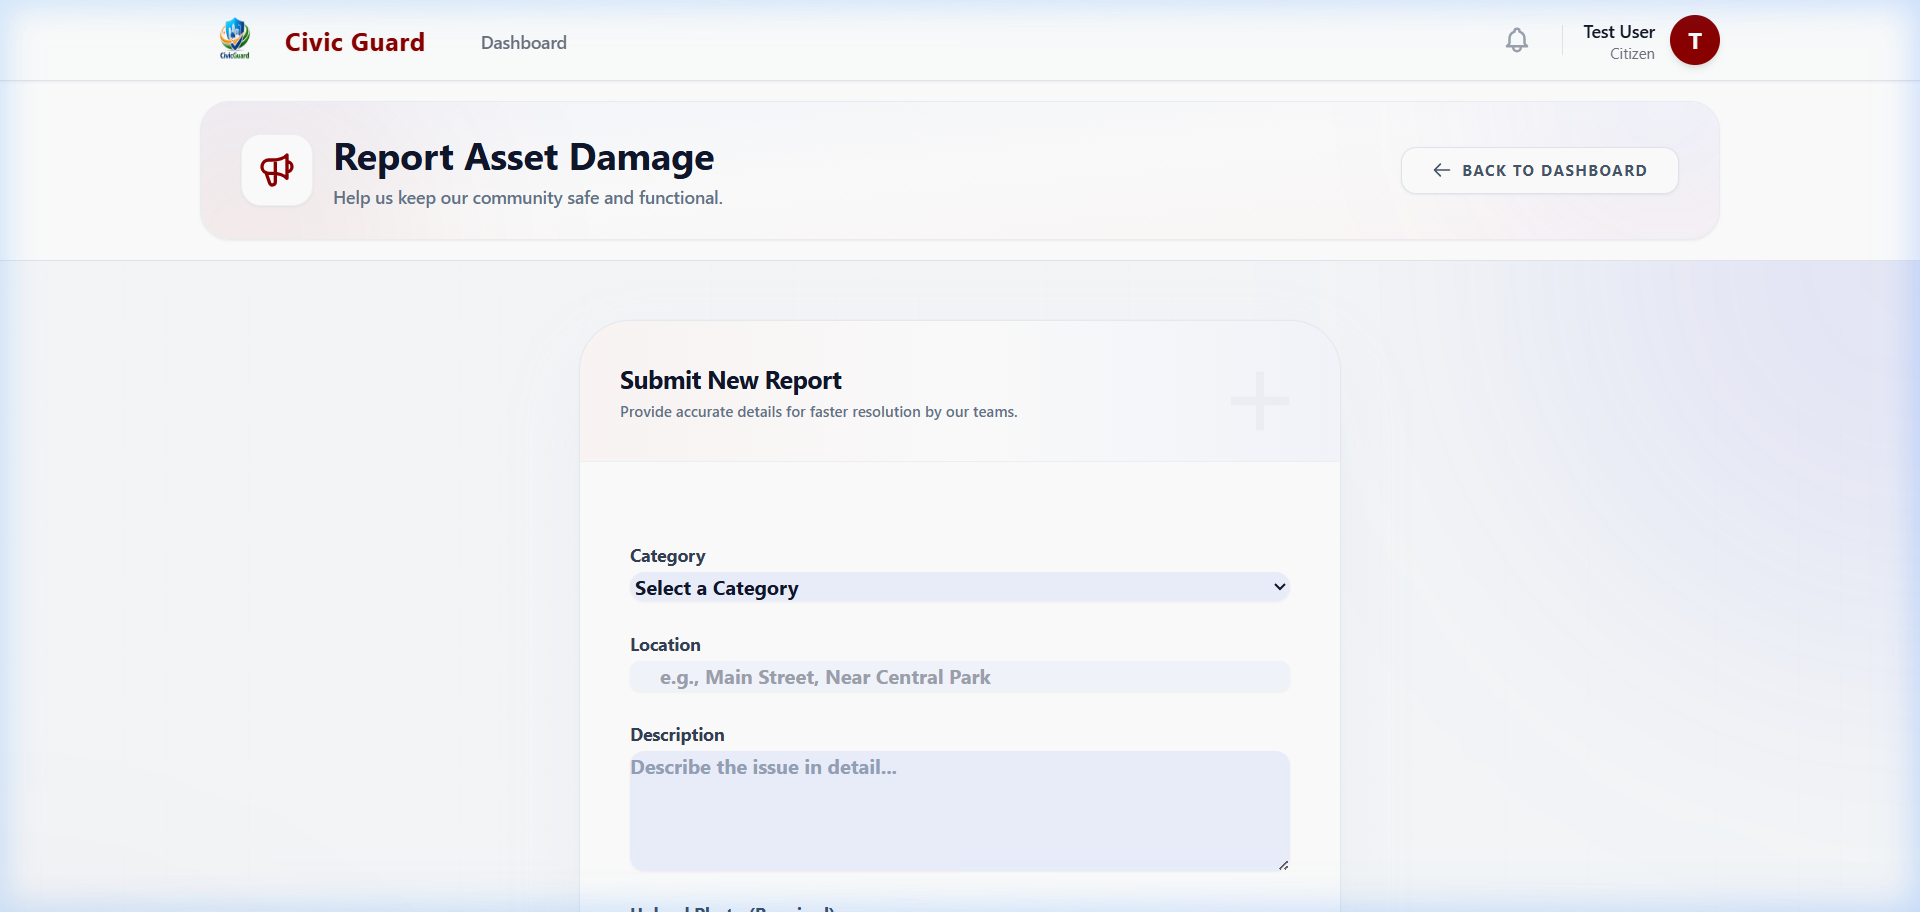
\includegraphics[width=0.9\textwidth]{images/report_creation.png}
    \caption{Implementation - Dynamic Report Submission Form}
\end{figure}

\subsection{Administrative Control Center}
The administrative and officer interfaces focus on data density and efficient task management.

\begin{figure}[H]
    \centering
    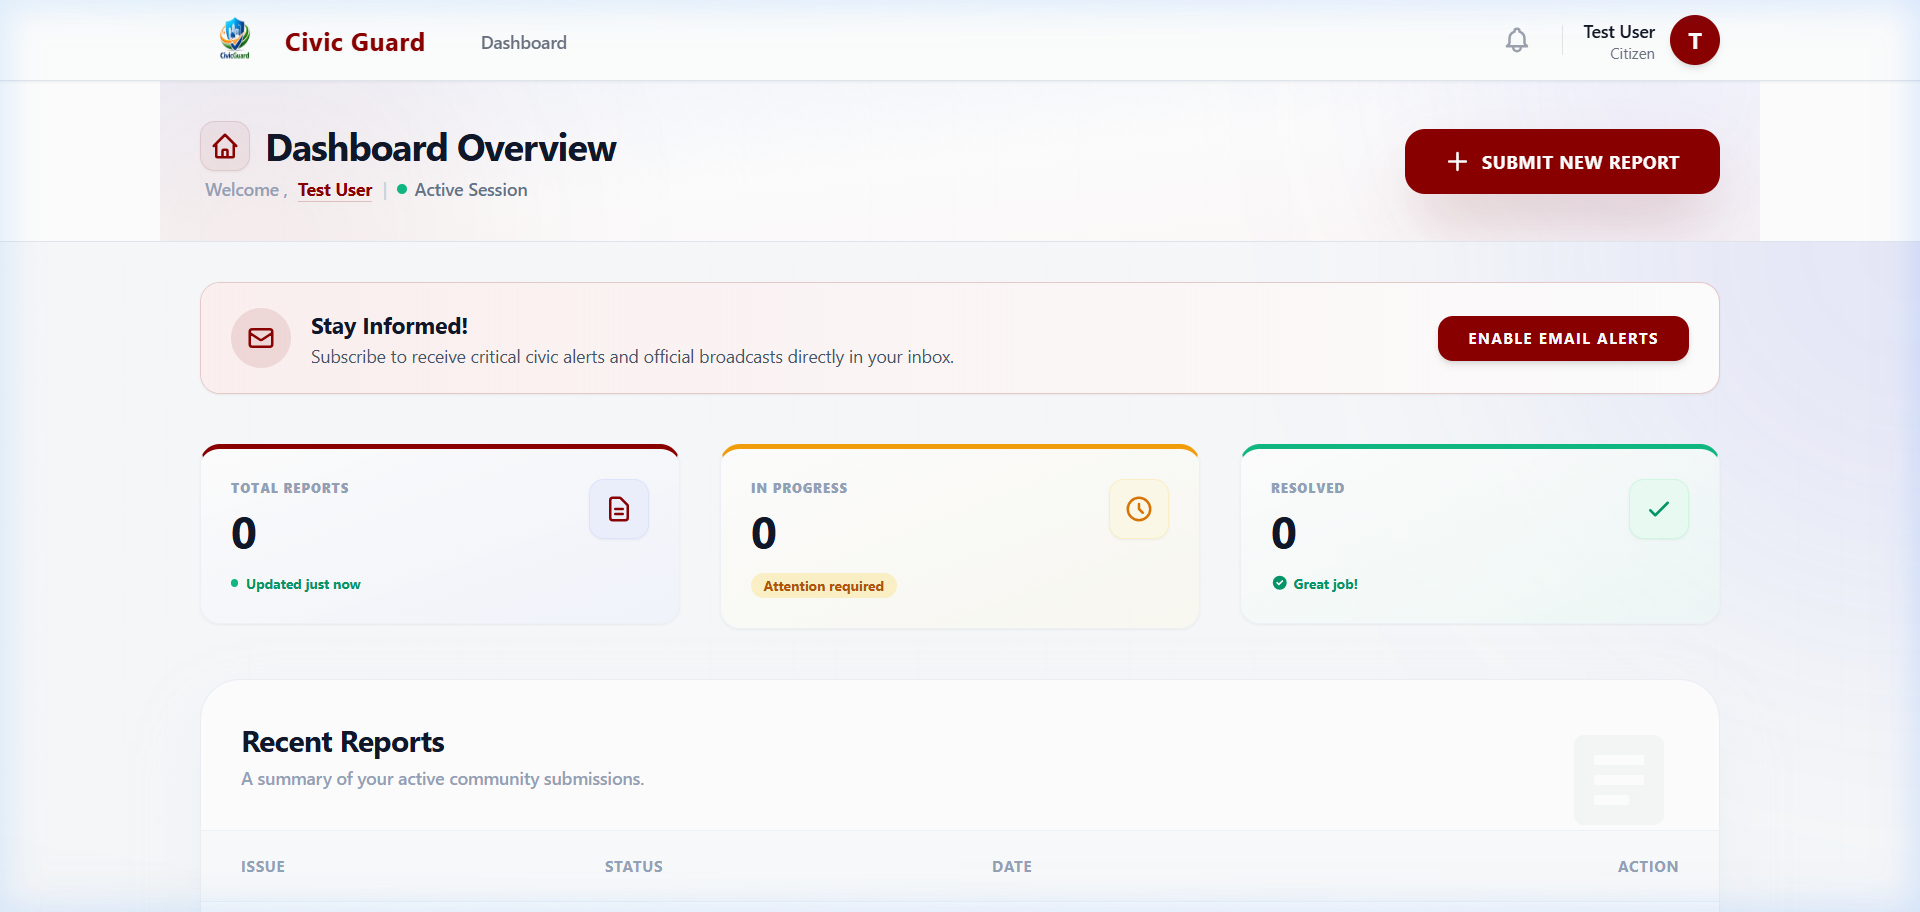
\includegraphics[width=0.9\textwidth]{images/dashboard_page.png}
    \caption{Implementation - Officer Task Management Interface}
\end{figure}
